\documentclass[12pt, a4paper]{article}
\usepackage[left=2.54cm, right=2.54cm, bottom=2.54cm, top=2.54cm]{geometry}
\linespread{1}
\usepackage{setspace}
\usepackage[utf8]{inputenc}
\usepackage{blindtext}
\usepackage[T1]{fontenc}
\usepackage{xcolor}
\usepackage{amsfonts}
\usepackage{amsmath}
\usepackage{amssymb}
\usepackage{fancyhdr}
\usepackage{tikz}
\pagestyle{fancy}
\fancyhead{}
\fancyfoot{}
\fancyfoot[R]{\thepage}
\renewcommand{\headrulewidth}{2pt}
\renewcommand{\footrulewidth}{2pt}
\usepackage{graphicx}
\usepackage{multicol}
\graphicspath{ {./img/} }

\title{Quiz 1 Kalkulus 1}
\date{}

\begin{document}

\maketitle
\begin{center}
Waktu       : 120 Menit  

Sifat       : Buku Tertutup
\end{center}

\vspace{20pt}
\textbf{Name \hspace{1.1 cm}:} Gilbran Mahdavikia Raja \\

\textbf{Student ID :} 5025241134 \\

\begin{center}
\vspace{20pt}
\noindent \textbf{Total: 120\%}

\vspace{40pt}
\begin{table}[h]
\centering
\begin{tabular}{|p{6 cm}|p{6 cm}|}
\hline
\rule{0pt}{30pt} \centering\textbf{Question} & \textbf{Score} \\ \hline
\rule{0pt}{30pt}\centering 1 (15\%) &   \\ \hline
\rule{0pt}{30pt}\centering 2 (10\%) &  \\ \hline
\rule{0pt}{30pt} \centering3 (10\%) &   \\ \hline
\rule{0pt}{30pt} \centering4 (10\%)  &  \\ \hline
\rule{0pt}{30pt}\centering 5 (20\%) &   \\ \hline
\rule{0pt}{30pt}\centering 6 (30\%) &   \\ \hline
\rule{0pt}{30pt}\centering 7 (25\%) &  \\ \hline
\rule{0pt}{30pt}\centering \textbf{Total} &   \\ \hline
\end{tabular}
\end{table}

\end{center}
\pagebreak

    % No 1
    \section{[\bf \textit{Simple Question} : 15\%] }
    
    Jawablah pertanyaan berikut ini dengan uraian jawaban yang singkat
    \begin{enumerate}
        \item[a] (5\%) Definisikan Nilai mutlak dari $v$
        \item[] \begin{enumerate}
            \item[] Definisi dari $|v|$ adalah $v$ bernilai $v$ apabila $v \geq 0$ dan $v$ bernilai $-v$ apabila $v < 0$ atau dapat juga dinotasikan dengan:
            
            \[\left\{ \begin{array}{rcl}v,& v\geq 0 \\ -v,& v < 0\end{array}\right.\]

        \end{enumerate}
        \vspace{1cm}
        \item[b] (5\%) Tuliskan 2 sifat dari Nilai Mutlak
        \item[] \begin{enumerate}
            \item[1.] $|x-y| = |y-x|$ 
            \item[2.] $|\frac{x}{y}| = \frac{|x|}{|y|}, y \neq 0$ 
        \end{enumerate}
        \vspace{1cm}
        \item[c] (5\%) Buatlah sketsa grafik $y + 6x = x^2 + 9$
        \item[] \begin{enumerate} \includegraphics[scale=0.3]{1c.png}\end{enumerate}
    \end{enumerate}
    \pagebreak

    % No 2
    \section{[{\bf Bilangan Real} : 10\%] }
    
    Selesaikan Persamaan berikut 
    
    \[ \frac{x-3}{x - 1} \le \frac{x}{x - 4} \]
    \begin{itemize}
        \item[$\Leftrightarrow$] $\frac{x-3}{x - 1}- \frac{x}{x - 4} \le 0$
        \item[$\Leftrightarrow$] $\frac{(x-3)(x - 4)-x(x-1)}{(x - 1)(x - 4)}\le 0$
        \item[$\Leftrightarrow$] $\frac{x^2-3x-4x+12-x^2+1x}{(x - 1)(x - 4)}\le 0$
        \item[$\Leftrightarrow$] $\frac{-6x+12}{(x - 1)(x - 4)}\le 0$
        \item[$\Leftrightarrow$] $\left\{ \begin{array}{rcl}-6x+12=0 \\ (x - 1)(x - 4)=0\end{array}\right.$
        \item[$\Leftrightarrow$] $\left\{ \begin{array}{rcl}x = 2\\x = 1\\x=4\end{array}\right.$
        \item[] \item[] 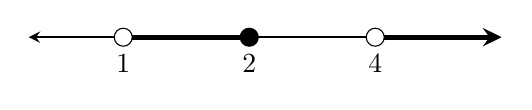
\begin{tikzpicture}[]
            \draw[thick,stealth-stealth] (-2,0) -- (4,0);
            \draw[line width=1.87pt] (-.8,0) -- (.8,0);
            \draw[line width=1.87pt, -stealth] (2.4,0) -- (4,0);
            \filldraw[fill=white] (-.8,0) circle (3.25pt) node[below,yshift=-.1cm] {$1$};
            \filldraw (.8,0) circle (3.25pt) node[below,yshift=-.1cm] {$2$};
            \filldraw[fill=white] (2.4,0) circle (3.25pt) node[below,yshift=-.1cm] {$4$};
        \end{tikzpicture}
        \item[$\Leftrightarrow$] $x\in (1,2]\cup(4,+\infty)$
    \end{itemize}
    \pagebreak

    % No 3
    \section{[{\bf Nilai Mutlak} :10\%]}
    
    Selesaikan Persamaan Nilai Mutlak berikut 
    
    \[\frac{2}{|x-3|} \le \frac{1}{x}\]
    \begin{itemize}
        \item[$\Leftrightarrow$] $\left\{ \begin{array}{rcl}x-3,& x-3> 0 \\ -x+3,& x-3 < 0\end{array}\right.$
        \item $\frac{2}{x-3} \leq \frac{1}{x},x> 3$
        \begin{itemize}
            \item[$\Leftrightarrow$] $2\le \frac{x-3}{x},x> 3$
            \item[$\Leftrightarrow$] $\frac{x-3}{x}-2\ge 0,x> 3$
            \item[$\Leftrightarrow$] $\frac{x-3-2x}{x}\ge 0,x> 3$
            \item[$\Leftrightarrow$] $\frac{-x-3}{x}\ge 0,x> 3$
            \item[$\Leftrightarrow$] $\varnothing$
        \end{itemize}
        \item $\frac{2}{-x+3} \leq \frac{1}{x},x< 3, x\neq 0$
        \begin{itemize}
            \item[$\Leftrightarrow$] $\frac{x-3}{x}\le -2,x< 3, x\neq 0$
            \item[$\Leftrightarrow$] $\frac{x-3}{x}+2\le 0,x< 3, x\neq 0$
            \item[$\Leftrightarrow$] $\frac{x-3+2x}{x}\le 0,x< 3, x\neq 0$
            \item[$\Leftrightarrow$] $\frac{3x-3}{x}\le 0,x< 3, x\neq 0$
            \item[] 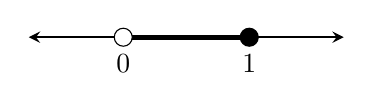
\begin{tikzpicture}[]
                \draw[thick,stealth-stealth] (-2,0) -- (2,0);
                \draw[line width=1.87pt] (-.8,0) -- (.8,0);
                \filldraw[fill=white] (-.8,0) circle (3.25pt) node[below,yshift=-.1cm] {$0$};
                \filldraw (.8,0) circle (3.25pt) node[below,yshift=-.1cm] {$1$};
            \end{tikzpicture}
        \end{itemize}
        \item[$\Leftrightarrow$] $x \in (0,1]$
    \end{itemize}
    \pagebreak

    % No 4
    \section{[{\bf Persamaan Garis} : 10\%]} 
    
    Tentukan persamaan garis $l$ yang melalui titik $(1,-1)$ jika diketahui bahwa garis $l$ sejajar dengan $2y + p^2x = 4$ dan tegak lurus dengan $x + py = 2$.
    \begin{itemize}
        \item $2y + p^2x = 4\longrightarrow m{\scriptscriptstyle 1}=-\frac{p^2}{2}$
        \item $x + py = 2\longrightarrow m{\scriptscriptstyle 2}=-\frac{1}{p}$
        \item $ml=m{\scriptscriptstyle 1} \longrightarrow ml = -\frac{p^2}{2}$
        \item $ml.m{\scriptscriptstyle 2} = -1$
        \begin{description}
            \item[$\Leftrightarrow$] $(-\frac{p^2}{2})(-\frac{1}{p}) = -1$
            \item[$\Leftrightarrow$] $p=-2$
        \end{description}
        \item $y-yl = m(x-xl)$
        \begin{description}
            \item[$\Leftrightarrow$] $y+1 = -\frac{2^2}{2}(x-1)$
            \item[$\Leftrightarrow$] $y+1 = -2(x-1)$
            \item[$\Leftrightarrow$] $y = -2x   +2-1$
            \item[$\Leftrightarrow$] $y = -2x+1$
        \end{description}
    \end{itemize}
    \pagebreak

    % No 5
    \section{[{\bf Persamaan Parabola} : 20\%]} 
    
    Felix melempar bola lurus ke atas dari ketinggian 4 meter di atas tanah pada saat waktu $t = 0$. Setelah $t$ detik jaraknya menjadi $s = 4 + 8t - t^2$ meter diatas tanah. Dapatkan
    \begin{enumerate}
        \item[a] (8\%) Grafik s terhadap t, dengan $t$ horizontal dan $s$ vertikal
        \begin{enumerate}
            \item[] $s(t)=4 + 8t - t^2$
            \item[] \includegraphics[scale=0.2]{5a.png}
        \end{enumerate}
        \item[b] (6\%) lama waktu bola saat mencapai ketinggian maksimum
        \begin{enumerate}
            \item[] $t{\scriptstyle maks}=-\frac{b}{2a}$
            \item[$\Leftrightarrow$] $t{\scriptstyle maks}=-\frac{8}{2(-1)}$
            \item[$\Leftrightarrow$] $t{\scriptstyle maks}=-\frac{8}{-2}$
            \item[$\Leftrightarrow$] $t{\scriptstyle maks}=4$
        \end{enumerate}
        \item[c] (6\%) tinggi maksimum bola tersebut dari atas tanah
        \item[] \begin{enumerate}
            \item[] $s{\scriptstyle maks} = s(t{\scriptstyle maks})$
            \item[$\Leftrightarrow$] $s(t{\scriptstyle maks})=4 + 8t{\scriptstyle maks} - t{\scriptstyle maks}^2$
            \item[$\Leftrightarrow$] $s(4)=4 + 8(4) - 4^2$
            \item[$\Leftrightarrow$] $s(4)=4 + 32 - 16 $
            \item[$\Leftrightarrow$] $s(4)=20 $
            \item[$\Leftrightarrow$] $s{\scriptstyle maks}=20$
        \end{enumerate}
    \end{enumerate}
    \pagebreak

    % No 6
    \section{[{\bf Fungsi Komposisi} : 30\%]} : 
    
    Diberikan fungsi $p(x) = \sqrt{x - 2}$ dan $q(x) = \frac{1}{x + 1}$. Dapatkan
    
    \begin{enumerate}
        \item[a] (6\%) Domain dan Range $p(x)$
        \item[]\begin{itemize}
            \item $\mathcal{D}(p)=[2,+\infty)$
            \item $\mathcal{R}(p)=(0,+\infty)$
        \end{itemize}
        \vspace{1cm}
        \item[b] (6\%) Domain dan Range $q(x)$
        \item[]\begin{itemize}
            \item $\mathcal{D}(q)=(-\infty,-1)\cup(-1,+\infty)$
            \item $\mathcal{R}(q)=(-\infty,0)\cup(0,+\infty)$
        \end{itemize}
        \vspace{1cm}
        \item[c] (9\%) Domain dan Range $p(q(x))$
        \item[] \begin{itemize}
            \item $\mathcal{D}(p\circ q)=\{x\in\mathcal{D}(q)\ |\ q(x) \in \mathcal{D}(p)\}$ 
            \begin{description}
                \item[$\Leftrightarrow$] $\mathcal{D}(p\circ q)=\{x\in(-\infty,-1)\cup(-1,+\infty)\ |\ \frac{1}{x + 1}\in[2,+\infty)\}$ 
                \item[$\Leftrightarrow$] $\mathcal{D}(p\circ q)\neq\mathcal{D}(q)$ 
                \item[$\Leftrightarrow$] $\mathcal{D}(p\circ q)= (-1,-\frac{1}{2}]$ 
            \end{description}
            \item $\mathcal{R}(p\circ q)=[0,+\infty)$
        \end{itemize}
        \vspace{1cm}
        \item[d] (9\%) Domain dan Range $q(p(x))$
        \item[] \begin{itemize}
            \item $\mathcal{D}(q\circ p)=\{x\in\mathcal{D}(p)\ |\ p(x) \in \mathcal{D}(q)\}$
            \begin{description}
                \item[$\Leftrightarrow$] $\mathcal{D}(q\circ p)=\{x\in(2,+\infty)\ |\ \sqrt{x - 2}\in(-\infty,-1)\cup(-1,+\infty)\}$ 
                \item[$\Leftrightarrow$] $\mathcal{D}(q\circ p)=\mathcal{D}(p)$ 
                \item[$\Leftrightarrow$] $\mathcal{D}(q\circ p)=[2,+\infty)$
            \end{description}
            \item $\mathcal{R}(q\circ p)=(0,1]$
        \end{itemize}
    \end{enumerate}
    \pagebreak

    % No 7
    \section{[{\bf Fungsi Invers} : 25\%]} 
    
    Diberikan fungsi $r(x) =  \sqrt{x + q} - p$ dan $s(x) = (x + p)^2 - q$ untuk sebarang bilangan real a dan b. Dapatkan 
    \begin{enumerate}
        \item[a] domain dan range  $r(x)$ agar fungsi $r(x)$ dan $s(x)$ saling invers
        \begin{itemize}
            \item $\mathcal{D}(r) = [-q,+\infty)$ 
            \item $\mathcal{R}(r) = [-p,+\infty)$ 
        \end{itemize}
        \item[b] domain dan range  $s(x)$ agar fungsi $r(x)$ dan $s(x)$ saling invers 
        \begin{itemize}
            \item $\mathcal{D}(r) = [-p,+\infty)$ 
            \item $\mathcal{R}(r) = [-q,+\infty)$ 
        \end{itemize}
        \item[c] sketsa kurva $r(x)$ dan $s(x)$ dalam satu bidang koordinat
        \begin{enumerate}
            \item[] $p = 0,q= -1$
            \item[] \includegraphics[scale=0.3]{7c.png}
        \end{enumerate}
    \end{enumerate} 
\end{document}